\subsection{Diseño Tridimensional del Armazón}

\par
Para el Diseño del armazón se tuvo que crear un modelo digital de las medidas del dispositivo, específicamente como el de la figura 4.30. En el programa fusion 360 este fue el resultado.

\begin{figure}[H]
	\centering
	\includegraphics[width=0.8\linewidth]{armazon00.png}
	\caption{Diseño Digital del prototipo (pantalla y circuito impreso)}
\end{figure}

\par \noindent
En la imagen 4.31 se pude apreciar el diseño de la pantalla de color rojo, el circuito impreso o placa en verde y podemos observar ciertos elementos de color negro. Dos de ellos sobresalen de la placa del prototipo; el cilíndrico vendría siendo la conexión del sensor de temperatura, jack de 3.5 mm y uno rectangular el cual sería el switch para encender o apagar el prototipo. Esto es muy importante que se encuentre en el modelo debido a que el armazón estará compuesto de dos moldes.  

\par \noindent
Un molde superior que cubrirá la pantalla y uno inferior que cubrirá el resto del prototipo. Ambos deben encapsular el arquetipo, tener las mismas dimensiones y debe contar con un mecanismo para que no se separen en caso de una caída por el usuario.

\subsubsection{Molde Superior}

\par 
El molde superior es la presentación del prototipo. Si se observa las imágenes 4.29 y 4.31, la pantalla LCD no es completamente plana. Posee ciertas dimensiones de altura que se deben tomar en cuenta. 

\par \noindent
Una regla general es que los modelos del armazón deben contar con un borde de menos de 2mm. Esto es para brindarle una base solida y una protección a los componentes. Lo primero que debió hacer es dibujos en plano del molde y todas sus partes.

\begin{figure}[H]
	\centering
	\includegraphics[width=0.5\linewidth]{armazon01.png}
	\caption{Dibujo del Area del Molde Superior}
\end{figure}

\begin{figure}[H]
	\centering
	\includegraphics[width=0.5\linewidth]{armazon04.png}
	\caption{Dibujo detallado de la pantalla LCD}
\end{figure}

\begin{figure}[H]
	\centering
	\includegraphics[width=0.6\linewidth]{armazon02.png}
	\caption{Dibujo del Area y bordes del circuito impreso o placa}
\end{figure}

\begin{figure}[H]
	\centering
	\includegraphics[width=0.6\linewidth]{armazon03.png}
	\caption{Dibujo de circunferencias para el uso de tornillos en el molde}
\end{figure}

\clearpage

\par \noindent
Ahora que se tiene definido los dibujos se procede a diseñar la parte superior.

\begin{figure}[H]
	\centering
	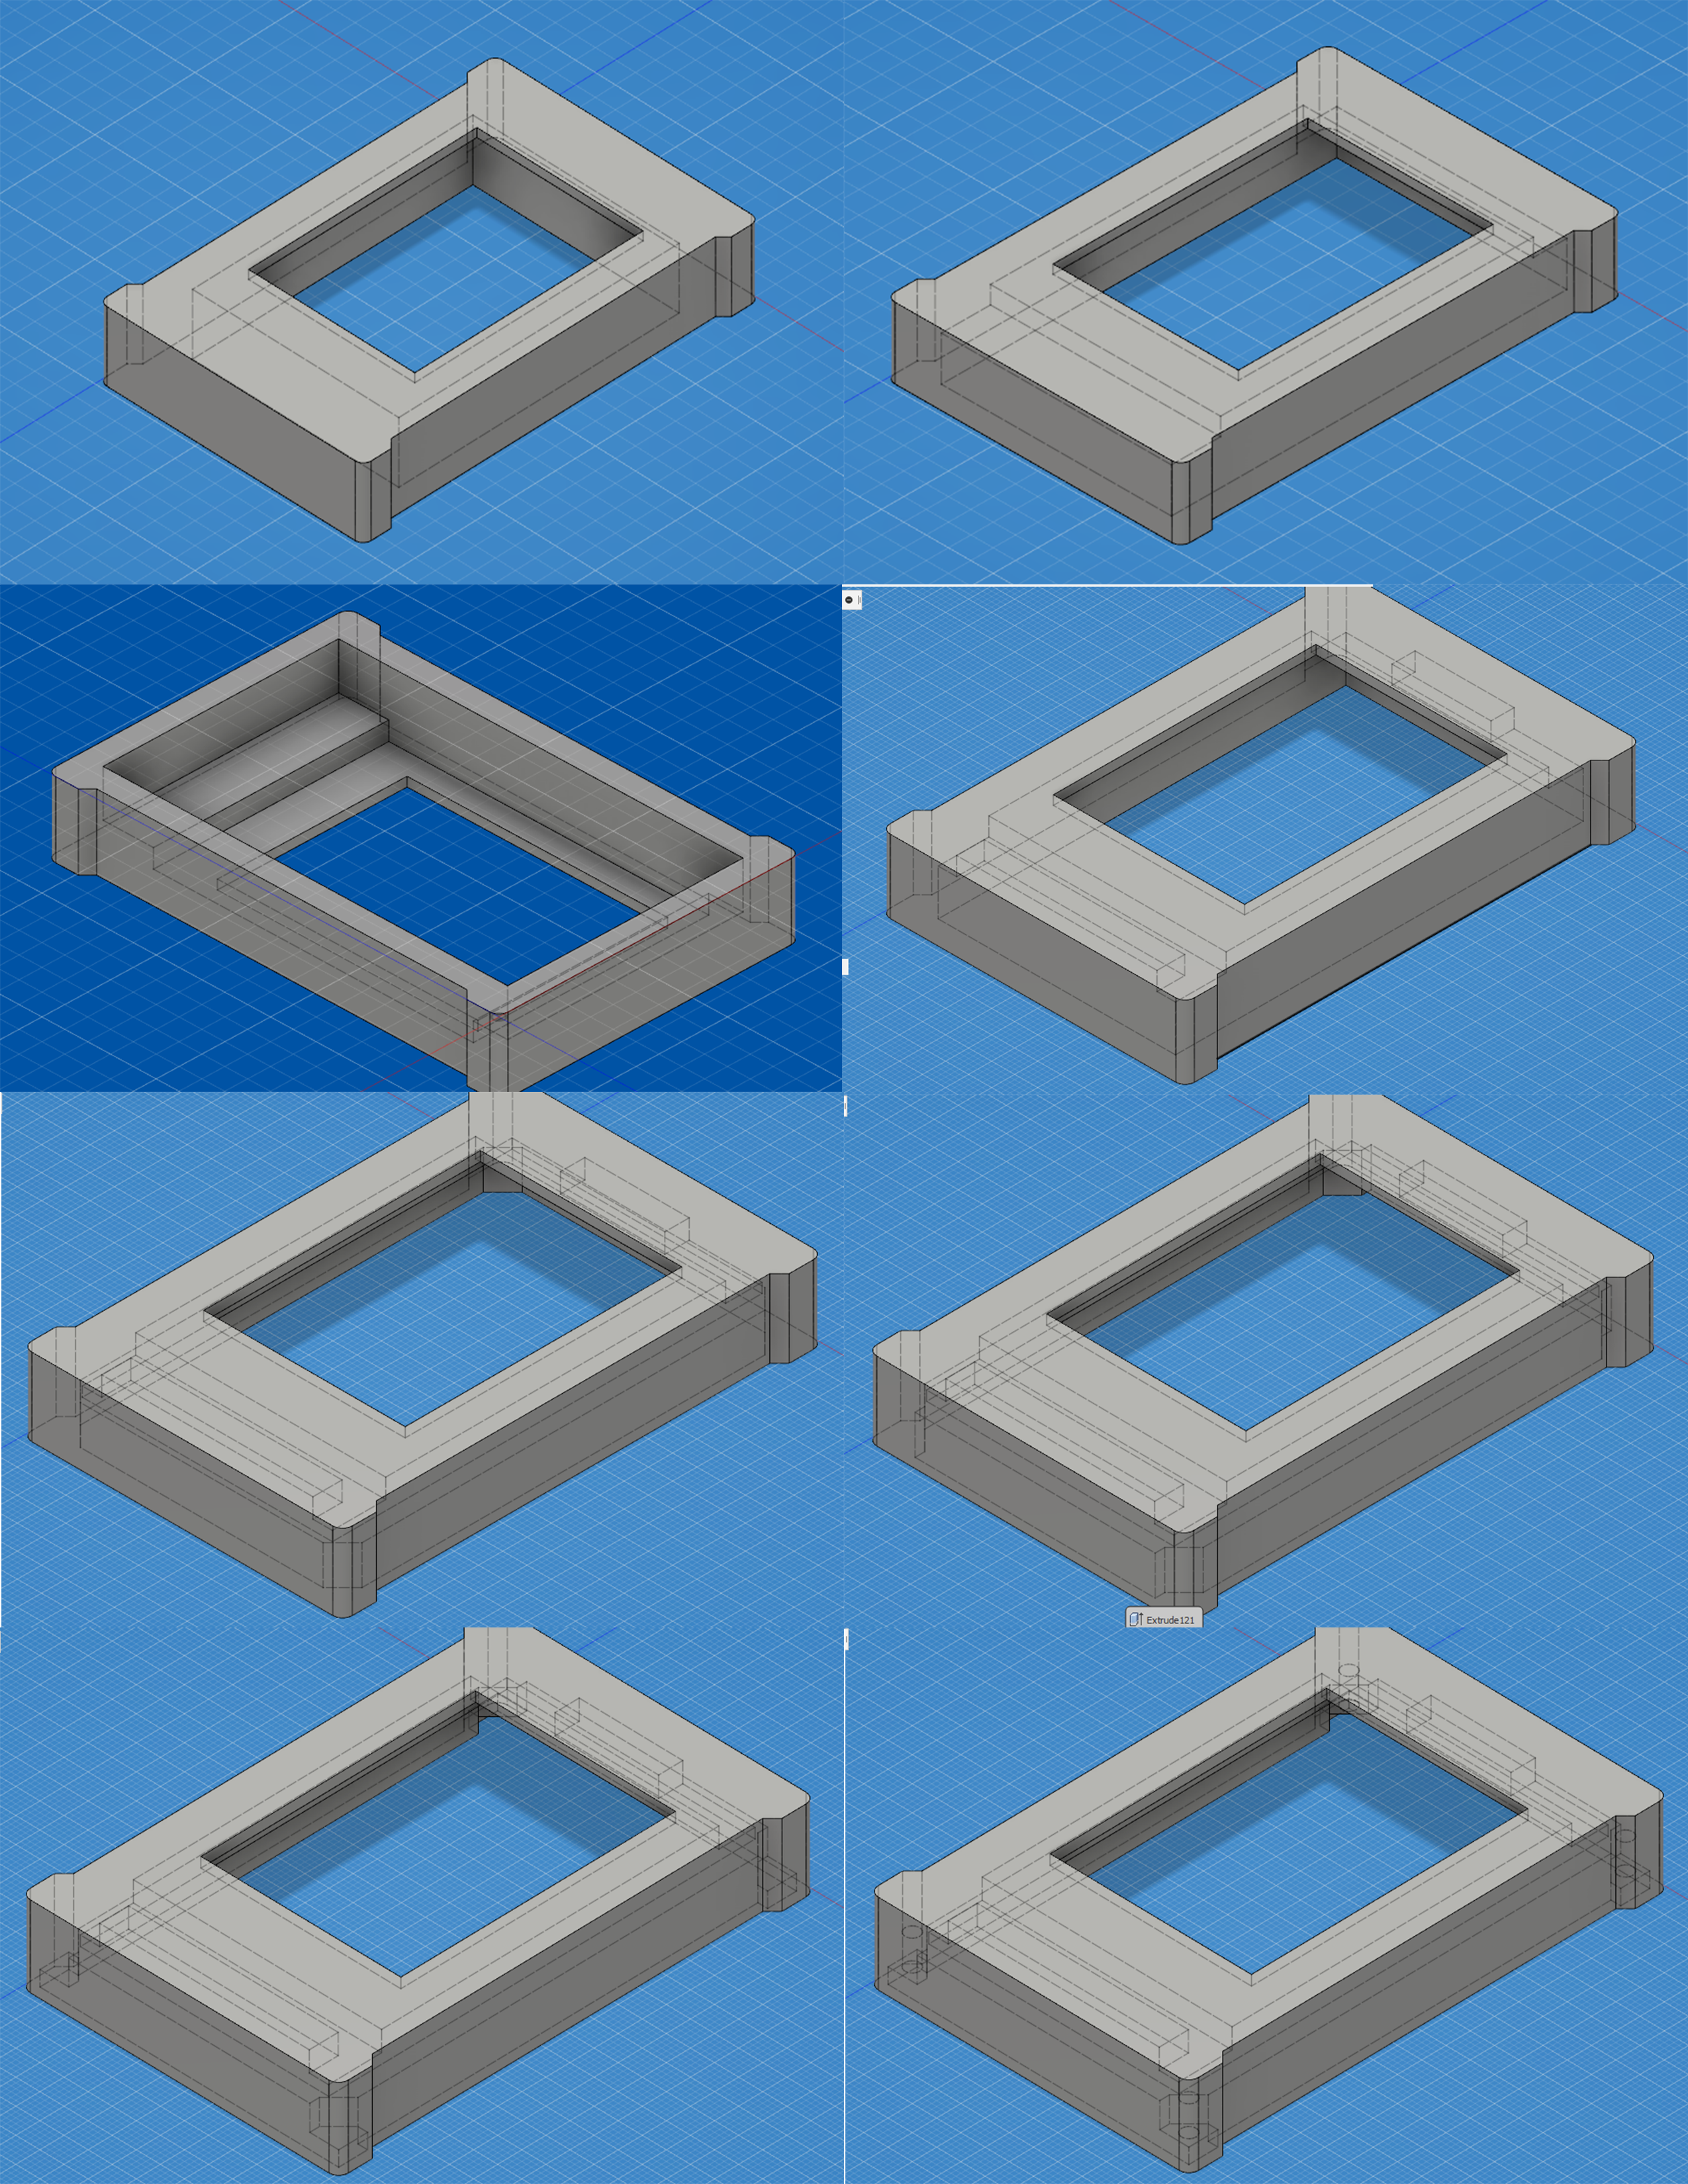
\includegraphics[width=0.8\linewidth]{armazon05.png}
	\caption{Proceso del Diseño del Molde Superior Parte 1}
\end{figure}

\par \noindent
En la figura 4.36 se puede ver los pasos en fusion 360. El diseño del molde superior empieza extrudiendo del dibujo de la figura 4.32; se subió el dibujo unos 17 mm y se creó el orificio donde se vera el LCD. A partir de allí se modelo la entrada para la pantalla y el espacio para la placa del prototipo. Una vez hecho eso en las esquinas se dejó un espacio diagonal; específicamente como en la figura 4.34, estos espacios tienen 3 mm de diferencia con el resto, esto es para insertar la otra pieza. Adicional se agregar los orificios donde se modeló la entrada de tornillos.

\begin{figure}[H]
	\centering
	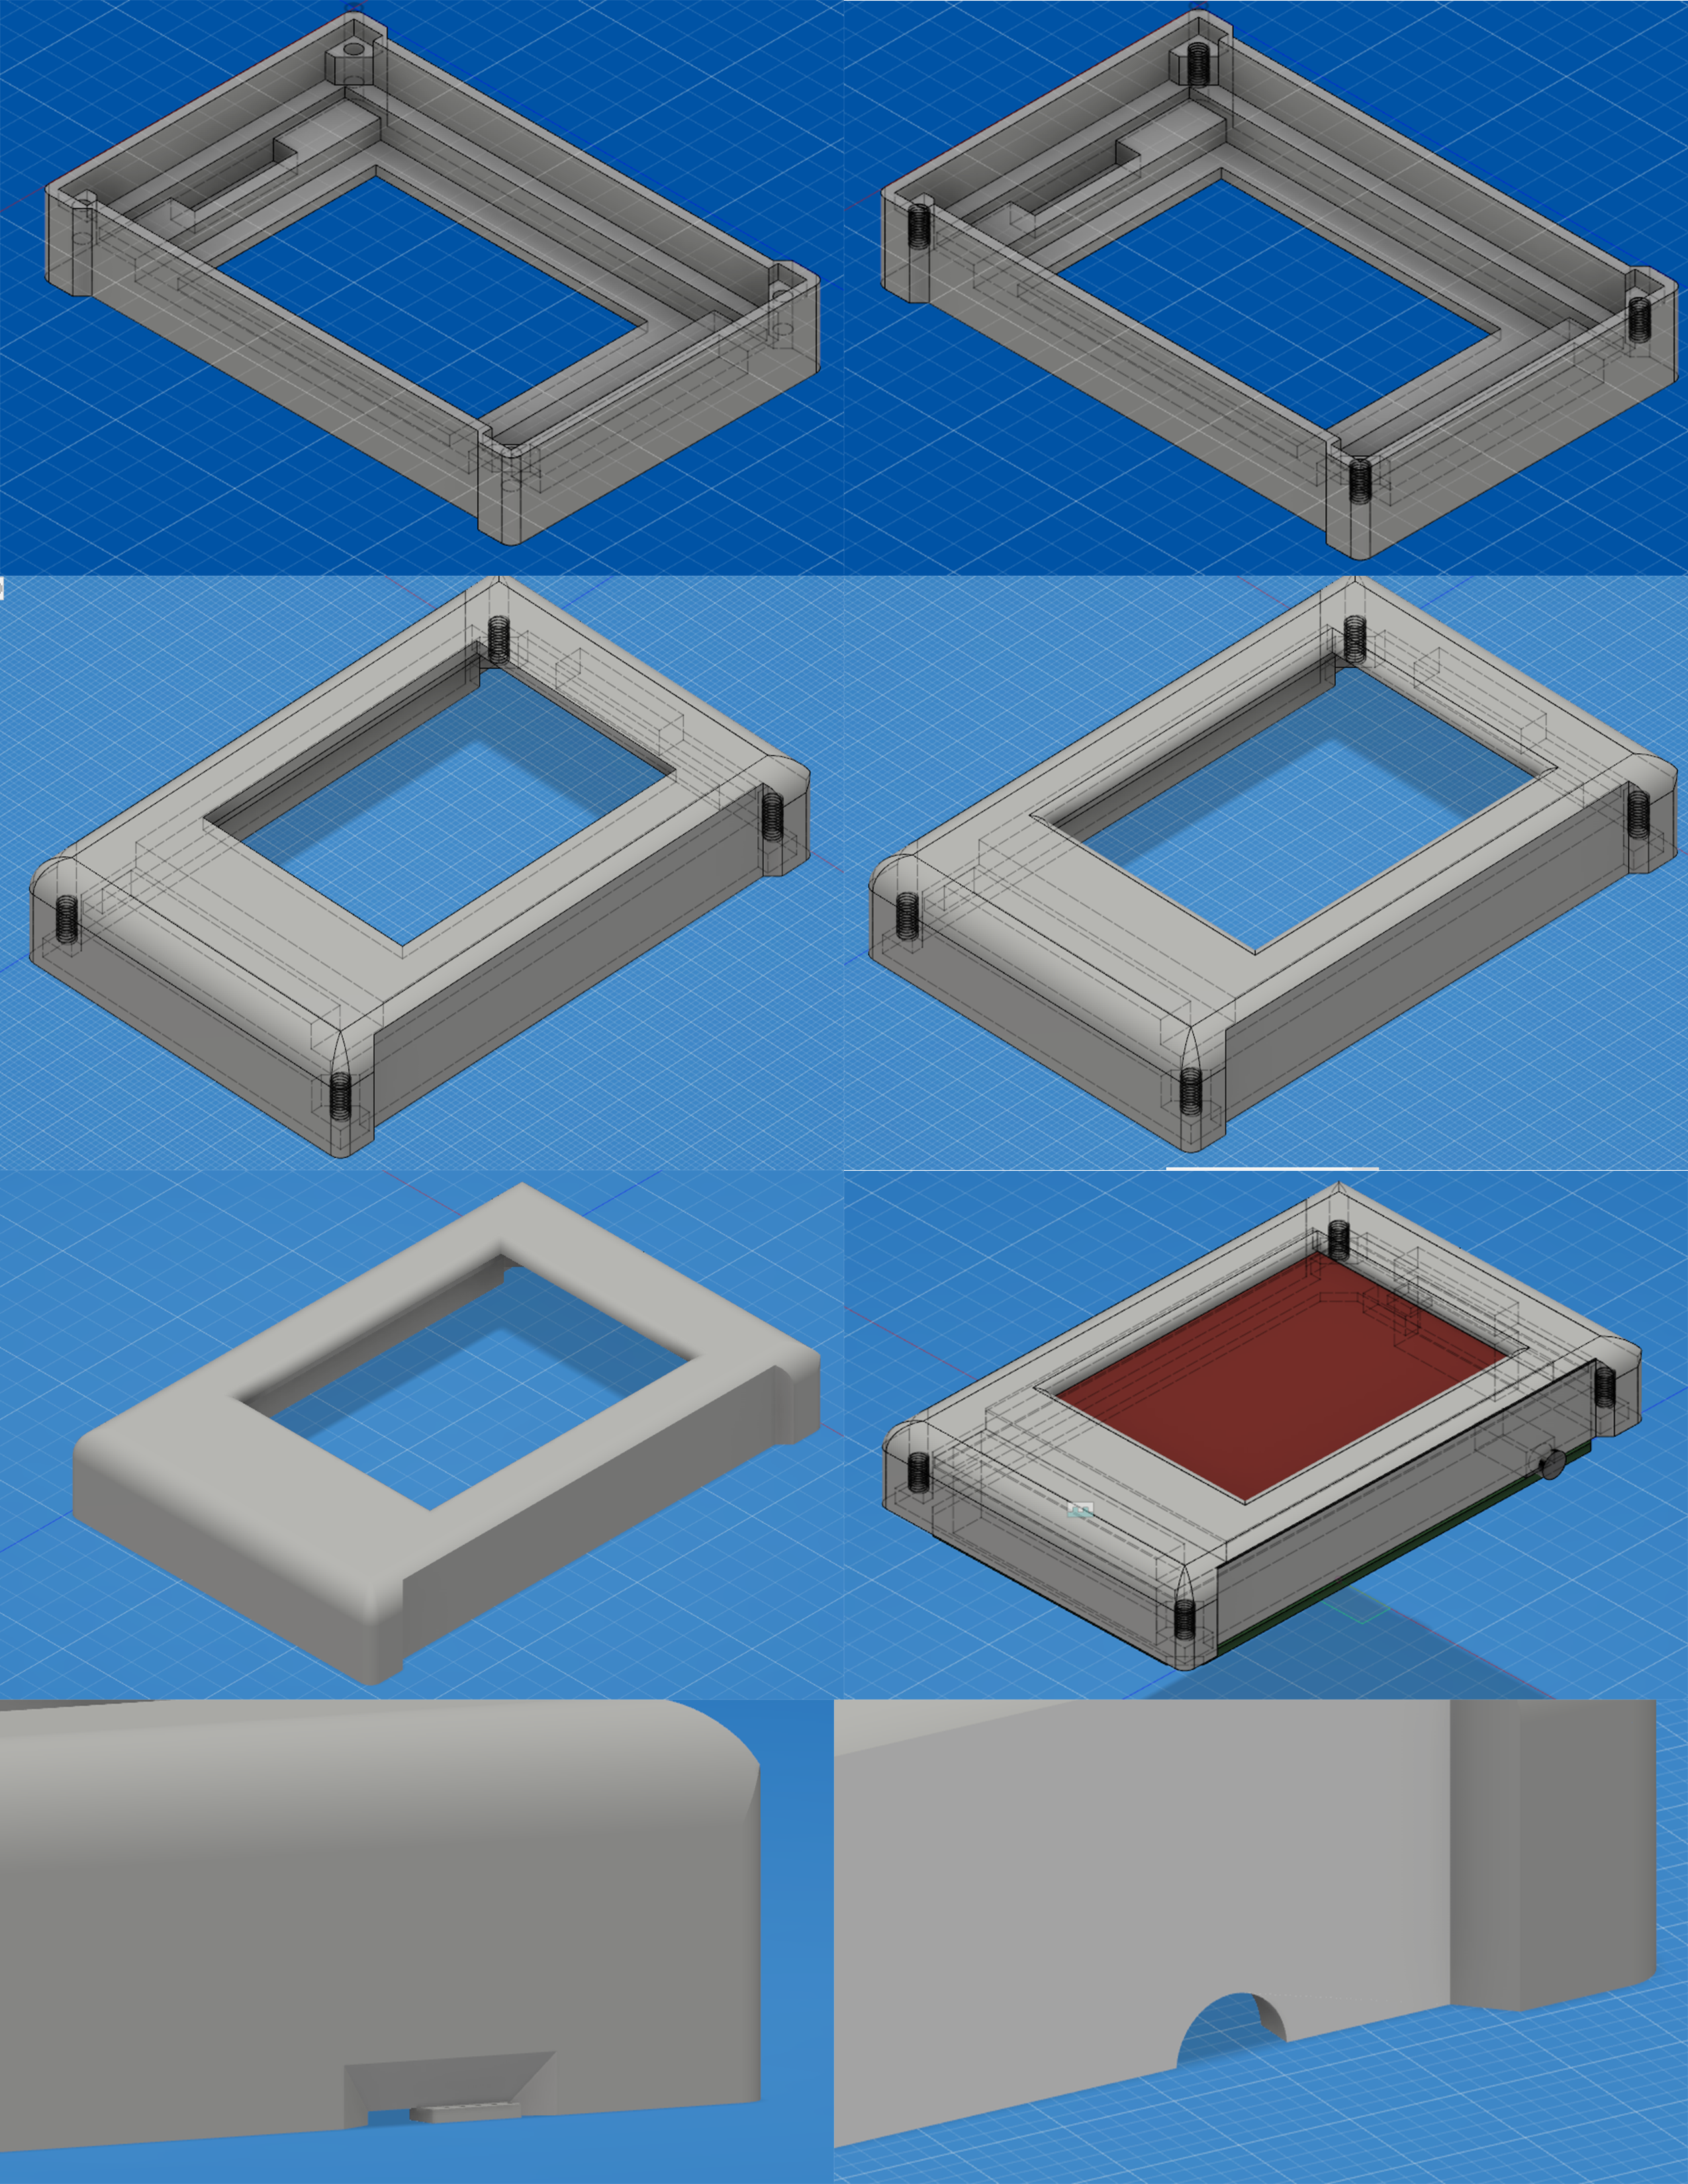
\includegraphics[width=0.8\linewidth]{armazon06.png}
	\caption{Proceso del Diseño del Molde Superior Parte 1}
\end{figure}

\par \noindent
En la figura 4.37 al inicio se aprecio todo lo que se hizo en la figura 4.36. Seguido se modelan las entradas para tornillos en los orificios de las esquinas. Los tornillos son de calibre M3. Realizado eso se suavizaron los bordes frontales para darle un aspecto mas profesional y por ultimo se cortarón los espacios para la entrada del sensor de temperatura y el interruptor de la batería. El resultado final es el siguiente.

\begin{figure}[H]
	\centering
	\includegraphics[width=0.8\linewidth]{armazon07.png}
	\caption{Diseño del molde superior finalizado}
\end{figure}

\par \noindent
Finalizado el diseño del molde superior procedemos a diseñar el molde inferior.

\subsubsection{Molde Inferior}

\par \noindent
El molde inferior es donde se encuentra la batería del prototipo y debe unirse a la pieza superior y cuenta con un espacio para que los tornillos entren. El molde se basó en los dibujos utilizados por el superior. 

\par \noindent
El molde inferior tiene una particularidad y es que tiene un espacio para un modulo de carga de la batería por lo que es necesario un corte para la entrada de micro-usb. 

\par \noindent
Observando la imagen 4.38 hay un corte de una circunferencia por donde se conectará el sensor de temperatura. El corte es a la mitad de la circunferencia para una inserción del dispositivo al armazón mas sencilla. Adicional hay un espacio en la parte superior del esqueleto para el interruptor de encendido del prototipo que también se encuentra a la mitad. En ambos cortes tuvo presente a el molde inferior. Para mantener la placa sin contacto directo con la batería y tener los cortes necesarios para las entradas del arquetipo se colocarón pequeños brazos para que la placa tenga donde sostenerse.

\begin{figure}[H]
	\centering
	\includegraphics[width=0.7\linewidth]{armazon08.png}
	\caption{Proceso del diseño del molde inferior parte 1}
\end{figure}

\begin{figure}[H]
	\centering
	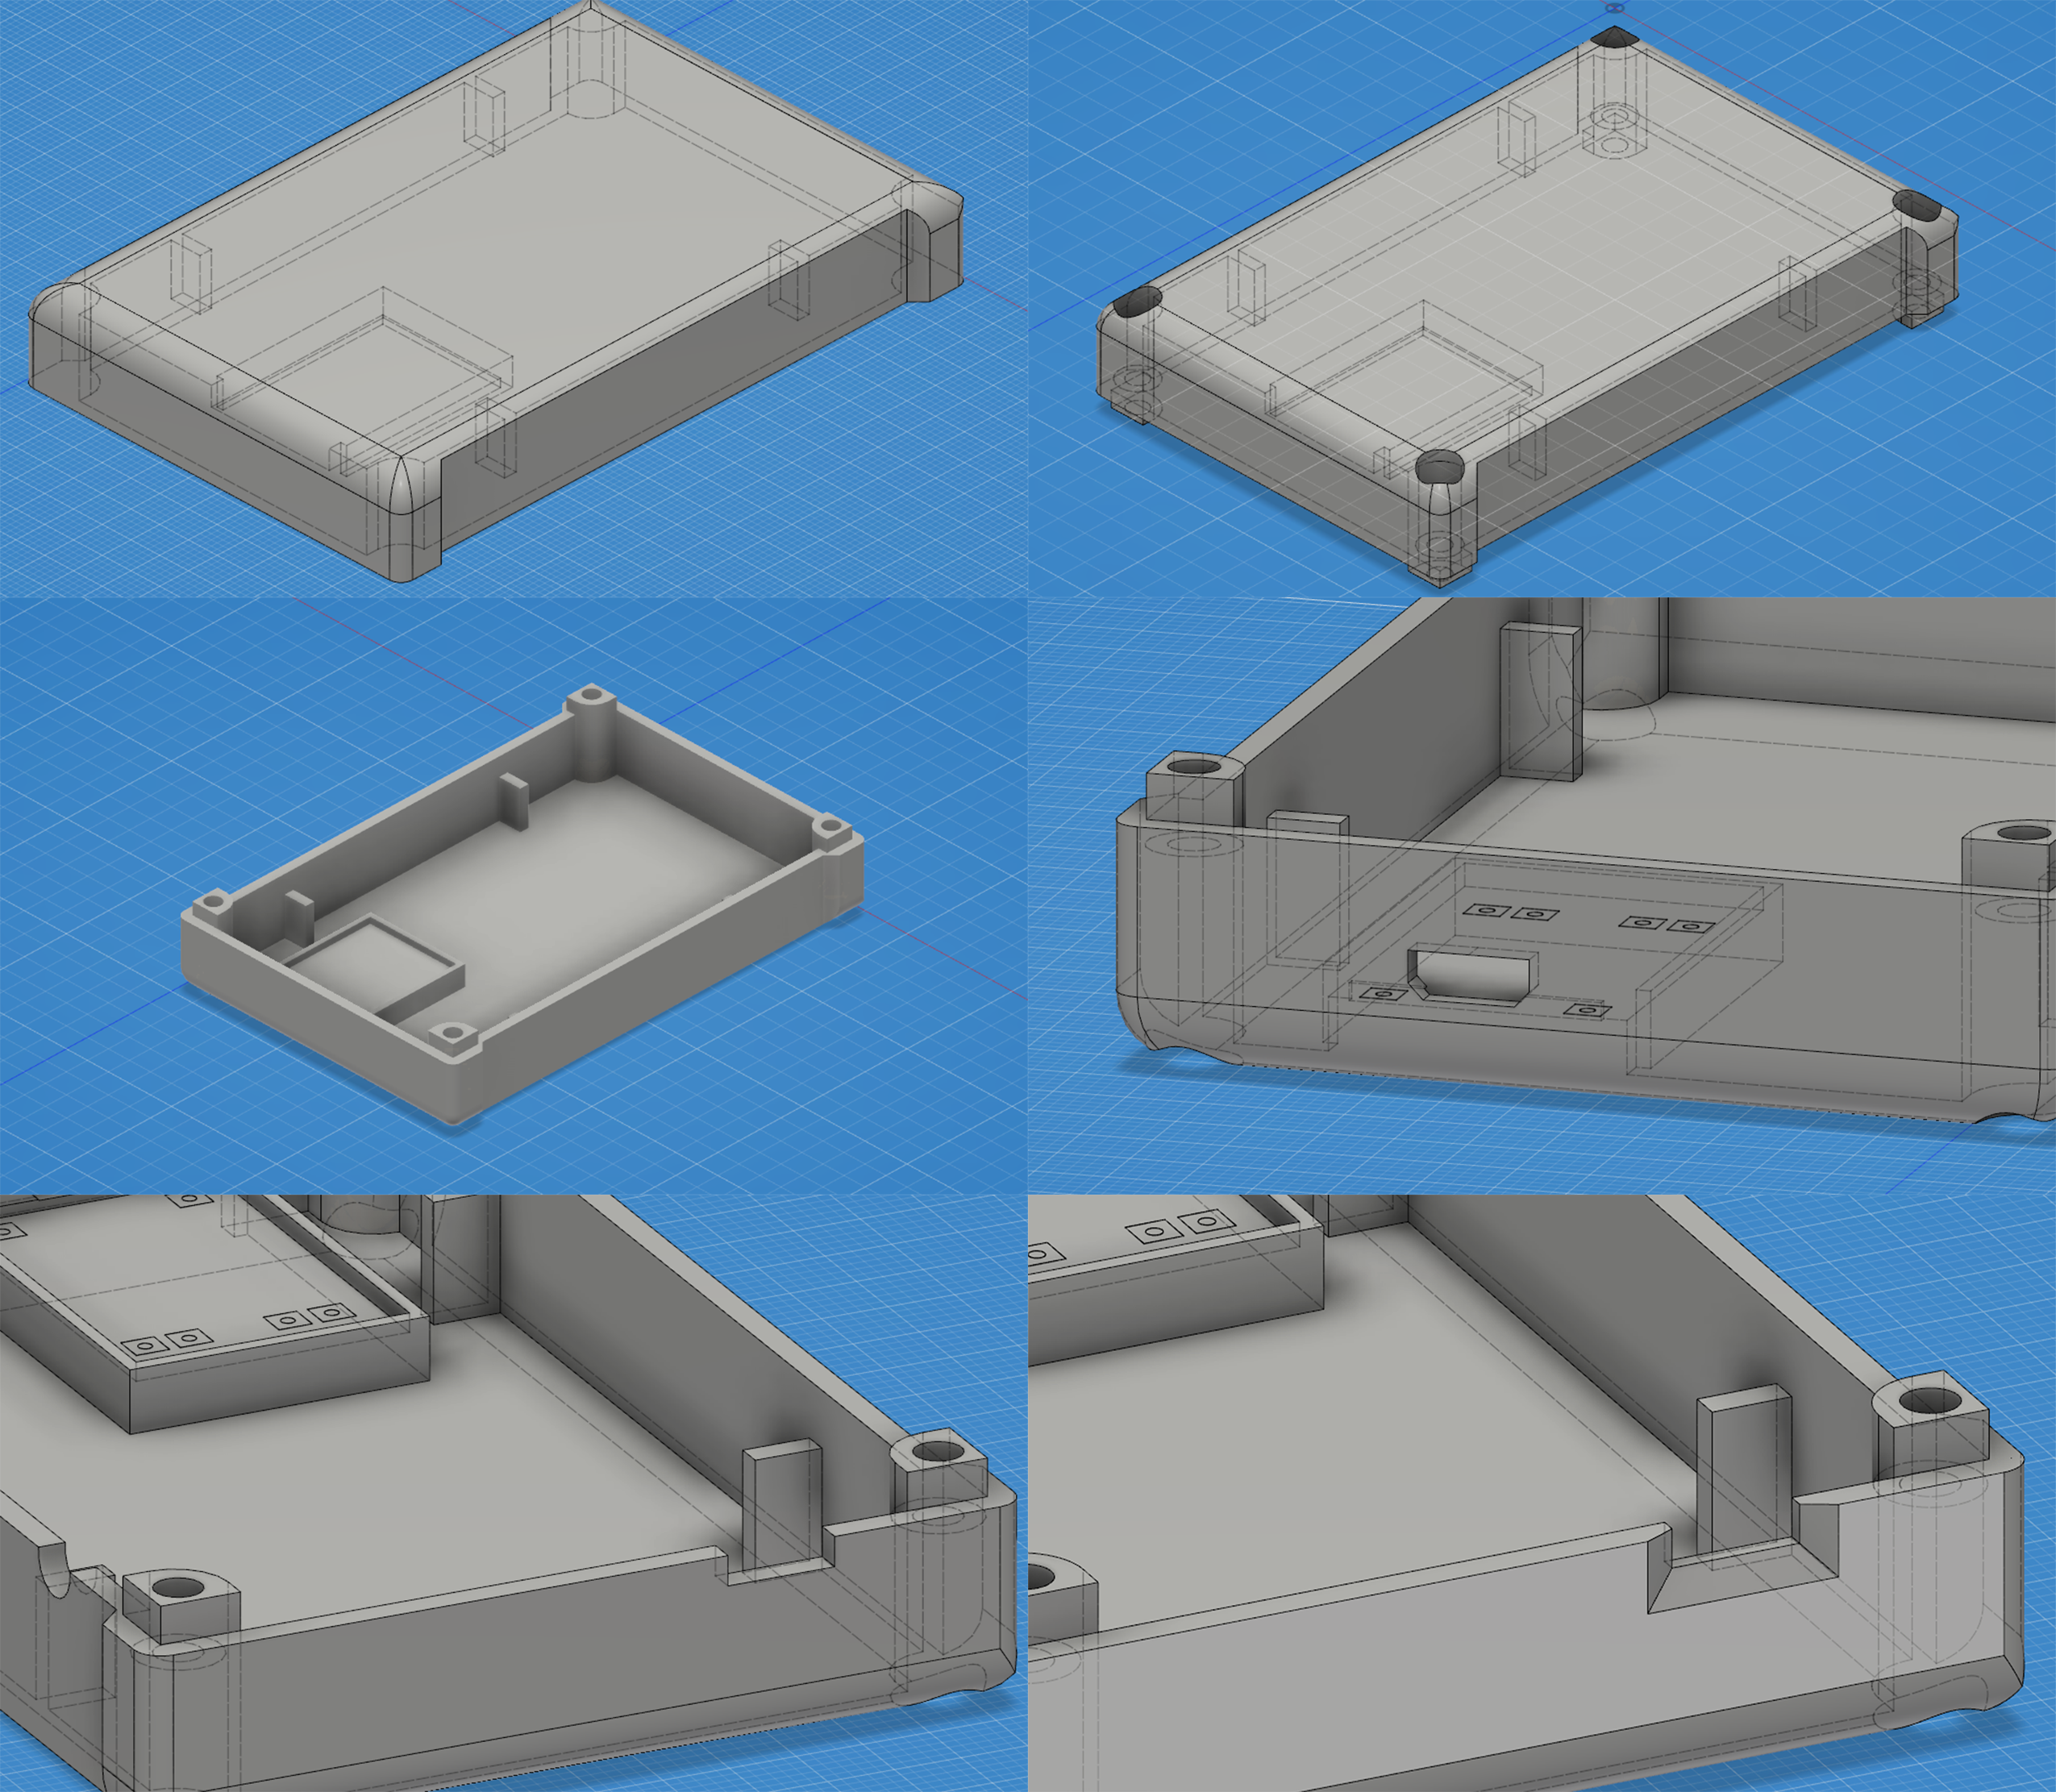
\includegraphics[width=0.7\linewidth]{armazon09.png}
	\caption{Proceso del diseño del molde inferior parte 2}
\end{figure}

\begin{figure}[H]
	\centering
	\includegraphics[width=0.8\linewidth]{armazon10.png}
	\caption{Diseño del molde inferior finalizado}
\end{figure}

\begin{figure}[H]
	\centering
	\includegraphics[width=0.8\linewidth]{armazon11.png}
	\caption{Diseño del final del armazón}
\end{figure}

\par \noindent
Una vez diseñado el molde superior e inferior se procedió a la impresión 3D de los mismos y el ensamblaje final.

